\def\SigleNumero{STT-1900}
\def\NomCours{Méthodes statistiques pour ingénieurs}
\def\DateEvaluation{18 octobre 2024}
\def\HeureEvaluation{18h30 à 21h20}
\def\Session{}
\def\NomEvaluation{Examen 1}
\def\Ponderation{40}
% Ne rien mettre entre les accolades si l'enseignant (ou l'enseignante) est aussi le coordonnateur (ou la coordonnatrice)
\def\Coordonnatrice{}
\def\Coordonnateur{}

% Ne rien mettre entre les accolades s'il y a plus d'une section
\def\Enseignant{}
\def\Enseignante{}

% Ne rien mettre entre les accolades s'il s'agit d'un cours à section unique
% Mettre le nom de chacun des enseignants et enseignantes entre les accolades
% Une case à cocher sera générée pour chacune des sections
\def\SectionA{Audrey-Anne Vallée}
\def\SectionB{Julien Miron}
\def\SectionC{}
\def\SectionD{}


\def\Directives{
\begin{enumerate}
\item Matériel autorisé:
\begin{itemize}
    \item Calculatrice scientifique {\bf autorisée par la faculté des sciences et de génie};
    \item Une seule feuille aide-mémoire \textbf{manuscrite} de format lettre (8.5''$\times$11'') recto-verso;
    \item Les tables de lois distribuées avec cet examen. S'il-vous-plaît, ne rien écrire sur celles-ci.
    \end{itemize}
\item Assurez-vous que cette évaluation comporte \numquestions ~questions réparties sur \numpages{}~pages, pour un total de \numpoints{}~points.\
\item \textbf{Veuillez ne pas dégrafer votre examen.}
\item Ajoutez vos initiales dans le bas de chaque page (sauf pour les tables de lois).
\item Vous devez\textbf{ justifier toutes vos réponses} par une démarche claire, sauf pour les questions à choix de réponse.\
\item Pour les questions à choix de réponse et les vrais ou faux, vous pouvez mettre un X, un crochet ($\checkmark$) ou remplir la case.\
\item Certains vrais ou faux demandent une justification. Aucun point ne sera donné sans justification, même si vous cochez la bonne réponse.
\item Pour les questions à choix de réponse, lorsqu'il est écrit «cochez tous les énoncés qui sont vrais/faux», il est possible qu'un seul énoncé soit vrai.
\item Le verso des feuilles peut être utilisé comme brouillon, \textbf{mais ne sera pas corrigé}. Attention à ne rien dégrafer.
\end{enumerate}
}



\documentclass{Evaluation}
\usepackage{multicol,graphicx}
\begin{document}

\newpage
%%%%%%%%%%%%%%%% QUESTION %%%%%%%%%%%%%%%%
\begin{questions}

\question\label{module1_1}  
On nous donne les probabilités suivantes:
\[
\begin{aligned}
    & P(A) = 0,45 \\
    & P(B) = 0,55 \\
    & P(C) = 0,1 \\
    & P(A\cap C) = 0 \\
    & P(B\cap C) = 0 \\
    & P(A | B) = 0,20 \\
    & 
\end{aligned}
\]

\begin{parts}
\part[3] Cochez tous les énoncés qui sont \textbf{vrais}. \textit{Chaque énoncé qui est coché alors qu'il ne devrait pas l'être annule les points d'un élément coché qui devrait l'être.}
\begin{checkboxes}
\correctchoice La probabilité du complément de $A$, $ P\left(\overline{A}\right) = 0,55 $.
\choice $P(A \cup B) = 1$.
\choice $A$, $B$ et $C$ sont mutuellement exclusifs.
\correctchoice $A$ et $C$ sont indépendants.
\choice Comme $P(A)+P(B)=1$, l'intersection de $A$ et $B$ est vide, c'est-à-dire $A\cap B = \emptyset$.
\vspace{0.1cm}
\end{checkboxes}

\vspace{0,5cm}

\part[4] \(A\) et \(B\) sont indépendants.

     \begin{oneparcheckboxes}
		\choice VRAI
		\correctchoice FAUX
\end{oneparcheckboxes}\\
{\bf Justification:}
\vspace{4cm}
\end{parts}




\begin{solution}

\end{solution}
\question[3] En analyse de survie, nous définissons la fonction de survie $S(x)$ comme étant la probabilité de survivre plus de $x$ unités de temps, c'est-à-dire $S(x)=P(X>x)$, où $X$ est une variable aléatoire continue qui mesure la durée de vie.  Soit la variable aléatoire $X$, dont la fonction de survie est donnée par 
\[ S(x) =
\begin{cases}
   \displaystyle e^{-x^2}& \text{si } x \ge 0, \\
    1 & \text{sinon}.
\end{cases}
\]

Laquelle des fonctions suivantes est la fonction de densité de $X$?

\begin{checkboxes}
\choice $f(x)=\left\{
			\begin{array}{ll}
   \displaystyle e^{-x^2}& \text{si } x \ge 0, \\
			0 & \mbox{sinon.}
			\end{array}
			\right. $
		\vspace{0.3cm}
\correctchoice $ f(x) = \left\{
			\begin{array}{ll}
   \displaystyle 2xe^{-x^2}& \text{si } x \ge 0, \\
			0 & \mbox{ sinon.}
			\end{array}
			\right. $
   		\vspace{0.3cm}
\choice $ f(x) = \left\{
			\begin{array}{ll}
   \displaystyle -2xe^{-x^2}& \text{si } x \ge 0, \\
			0 & \mbox{ sinon.}
			\end{array}
			\right. $
   		\vspace{0.3cm}
\choice $ f(x) = \left\{
			\begin{array}{ll}
   \displaystyle 1-e^{-x^2}& \text{si } x \ge 0, \\
			0 & \mbox{sinon.}
			\end{array}
			\right. $
   		\vspace{0.3cm}

\choice $ f(x) = \left\{
			\begin{array}{ll}
   \displaystyle 1-e^{-2x}& \text{si } x \ge 0
   , \\

			0 &  \mbox{ sinon. }
			\end{array}
			\right. $

      		\vspace{0.3cm}

\choice Nous ne pouvons pas déterminer la fonction de densité à partir des informations données.

\end{checkboxes}
\newpage

\question[3]\label{normaleBivariee}
Laquelle des fonctions suivantes est une fonction de répartition? 

\begin{checkboxes}
\choice $F(a)=\left\{
			\begin{array}{ll}
			a  & \mbox{ si } a \ge 0, \\
			0 & \mbox{sinon.}
			\end{array}
			\right. $
		\vspace{0.3cm}
\correctchoice $ F(b) = \left\{
			\begin{array}{ll}
			0  & \mbox{ si } b<0, \\
			\displaystyle \sfrac{b}{2} & \mbox{ si } 0\leq b < 2,\\
			0 & \mbox{ si } b \geq 2.
			\end{array}
			\right. $
\choice $ F(c) = \left\{
			\begin{array}{ll}
			\sqrt{c}  & \mbox{ si } 0\leq c\leq 1, \\
			0 & \mbox{sinon.}
			\end{array}
			\right. $
\choice $ F(d) = \left\{
			\begin{array}{ll}
			0  & \mbox{ si } d < 0, \\
			d & \mbox{ si } 0 \leq d \leq 1,\\
			1 &  \mbox{ si } d > 1.
			\end{array}
			\right. $

   \choice $ F(e) = \left\{
			\begin{array}{ll}
			0  & \mbox{ si } e < 0, \\
			e & \mbox{ si } 0 \leq e \leq 1,\\
                1-e & \mbox{ si } 1< e \leq 2,\\ 
			1 &  \mbox{ si } e> 2.
			\end{array}
			\right. $
\end{checkboxes}

\question\label{module1_2} 
Dans une usine, deux machines, A et B, produisent des composants. La machine A produit les trois quarts des composants et la machine B produit le reste. Un quart des composants produits dans l'usine sont défectueux. Lorsqu'un composant est choisi au hasard, sa probabilité d'avoir été produit par la machine A et d'être défectueux est d'un sixième. 

\begin{parts}
    \part[3] Tracez le diagramme de Venn qui représente cette situation. \textit{Vous n'avez qu'à identifier les événements. Il n'est pas nécessaire d'inscrire les probabilités.}
    \vspace{5cm}

    \part[4] Si un composant est défectueux, quelle est la probabilité qu'il ait été produit par la machine B?
\end{parts}
\begin{solution}
Soit \( D \) l'événement qu'un composant soit défectueux et \( A \) l'événement qu'il ait été produit par la machine A et \( B \) l'événement qu'il ait été produit par la machine B.

Nous cherchons \( P(B|D) \).

Les données fournies sont:
\[ P(A) = 0,75 = 3/4\]
\[ P(B) = 0,25 =1/4\]
\[ P(D) = 0,25 = 1/4 \]
\[ P(D \cap A) = 1/6 \]


On cherche
\[ P(B|D) = \frac{P(B \cap D)}{P(D)} .\]

Calculons \(P(B \cap D)\) en utilisant la loi des probabilités totales:
\[ P(D) = P(D\cap A)  + P(D \cap B) \]
\[ 1/4 = 1/6 + P(D \cap B) \]
\[ P(D \cap B) = 1/4 - 1/6 = \frac{6-4}{24} = 1/12) \]

Alors:
\[ P(B|D) = \frac{P(B \cap D)}{P(D)} .\]
\[ P(B|D) = \frac{1/12}{1/4} = 1/3 .\]
\end{solution}



\vspace{0.5cm}

\newpage

\question Soit deux échantillons aléatoires indépendants provenant de populations normales, tels que:
\begin{align*}
    X_1,\hdots,X_{16}&\sim\mathcal{N}(7, 4),\\
    Y_1,\hdots,Y_{100}&\sim\mathcal{N}(8, 9).
\end{align*}

\begin{parts}
    \part[2] Quelle est la loi de $A=X_1+X_2+X_3$?
    \begin{checkboxes}
        \choice $A\sim\mathcal{N}(7; 4)$
        \choice $A\sim\mathcal{N}(7; 12)$
        \choice $A\sim\mathcal{N}(7; 36)$
        \choice $A\sim\mathcal{N}(21; 4)$
        \choice $A\sim\mathcal{N}(21; 12)$
        \choice $A\sim\mathcal{N}(21; 36)$
        \choice Aucune de ces réponses
    \end{checkboxes}

    \part[2] Quelle est la loi de $B=\displaystyle\frac{1}{16}\sum_{i=1}^{16}X_i$?
        \begin{checkboxes}
        \choice $B\sim\mathcal{N}(0,4375; 4)$
        \choice $B\sim\mathcal{N}(0,4375; 0,25)$
        \choice $B\sim\mathcal{N}(0,4375; 1)$
        \choice $B\sim\mathcal{N}(7; 4)$
        \choice $B\sim\mathcal{N}(7; 0,25)$
        \choice $B\sim\mathcal{N}(7; 1)$
        \choice Aucune de ces réponses
    \end{checkboxes}

    \vspace{0.25cm}
    \part[2] Quelle est la loi de $C=X_1-Y_1$?
        \begin{checkboxes}
        \choice $C\sim\mathcal{N}(-1; -5)$
        \choice $C\sim\mathcal{N}(-1; 13)$
        \choice $C\sim\mathcal{N}(-1; 97)$
        \choice $C\sim\mathcal{N}(15; -5)$
        \choice $C\sim\mathcal{N}(15; 13)$
        \choice $C\sim\mathcal{N}(15; 97)$
        \choice Aucune de ces réponses
    \end{checkboxes}
   \part[2] Quelle est l'espérance de $D=\displaystyle\frac{\overline{Y}-8}{S_Y/10}$, où $S_Y$ est l'écart-type échantillonnal de $Y$?
        \begin{checkboxes}
        \choice $E(D)=8$
        \choice $E(D)=100$
        \choice $E(D)=99$
        \choice $E(D)=0$
        \choice $E(D)=15$
        \choice $E(D)=800$
        \choice Aucune de ces réponses
    \end{checkboxes}
\end{parts}
\newpage

\vfill

\question[10]
Déterminez si les énoncés suivants sont vrais ou faux. 

\textbf{\textit{Une bonne réponse vaut 2 points, une mauvaise réponse vaut -1 point et une réponse vide vaut 0 point, pour un total minimum de 0 point.}}

\begin{parts}
    \part Si $X_1,\hdots,X_{100}$ constituent un échantillon aléatoire simple issu d'une loi quelconque d'espérance $\mu=0$ et de variance $\sigma^2=100^2$, alors la moyenne échantillonnale de ces 100 valeurs suit approximativement une loi normale centrée-réduite. 

    \begin{oneparcheckboxes}
        \choice Vrai
        \correctchoice Faux
    \end{oneparcheckboxes}

    \begin{solution}
        Faux
    \end{solution}
    \vspace{0.25cm}
    \part Si $X_1,\hdots,X_{17}$ constituent un échantillon aléatoire simple issu d'une loi $\mathcal{N}(5; 4)$, alors la variable $4S^2$ a une espérance de 16 et une variance de 32. 

    \begin{oneparcheckboxes}
        \choice Vrai
        \correctchoice Faux
    \end{oneparcheckboxes}
        \begin{solution}
        Vrai
    \end{solution}
        \vspace{0.25cm}

    \part Si $W$ suit une $\chi^2_4$ (khi-carré avec $4$ degrés de liberté), alors $P(W>4)=P(W<4)$. 

    \begin{oneparcheckboxes}
        \choice Vrai
        \correctchoice Faux
    \end{oneparcheckboxes}
    
    \begin{solution}
        Faux
    \end{solution}
        \vspace{0.5cm}
    \item Le poids des tomates d'un certain agriculteur suit une loi normale de moyenne $300\text{ grammes}$ et de variance $100\text{ grammes}^2$. On prend des mesures sur 25 tomates choisies aléatoirement et on obtient une moyenne échantillonnale de $309,12\text{ grammes}$ et une variance échantillonnale de $118,3\text{ grammes}^2$. Dans cette situation, les nombres $309,12$ et $118,3$ sont des paramètres et les nombres $300$ et $100$ sont des statistiques.
    
    \begin{oneparcheckboxes}
        \choice Vrai
        \correctchoice Faux
    \end{oneparcheckboxes}
            \begin{solution}
        Vrai
    \end{solution}
        \vspace{0.5cm}


    \part Soit deux échantillons aléatoires indépendants de taille $n=26$ et $m=26$ qui proviennent de lois normales $\mathcal{N}(\mu_X, \sigma_X^2)$ et $\mathcal{N}(\mu_Y, \sigma_Y^2)$. Les moyennes échantillonnales sont respectivement $\overline{X}$ et $\overline{Y}$, alors que les variances échantillonnales sont respectivement $S^2_X$ et $S^2_Y$. La statistique ${\displaystyle S^2_X}/ {\displaystyle S^2_Y}$ suit une $F_{25,25}$. 

    \begin{oneparcheckboxes}
        \choice Vrai
        \correctchoice Faux
    \end{oneparcheckboxes}
    
            \begin{solution}
        Vrai
    \end{solution}

    \end{parts}
\question[4]\label{micro}
Soit les 21 valeurs suivantes:

\begin{center}
\begin{tabular}{  c c c c c c c c }
111  &112  &112  &112  &113  &113  &113 \\
113 &115  &115  &115  &115 &115 & 116 \\
118 & 118 & 118 & 119 & 124 &124 & 125\\
\end{tabular}
\end{center}

Le diagramme en boîte ci-dessous a été tracé à partir de ces résultats. Il y a toutefois une erreur (il ne s'agit pas d'un titre ou de noms d'axes).

\begin{center}
		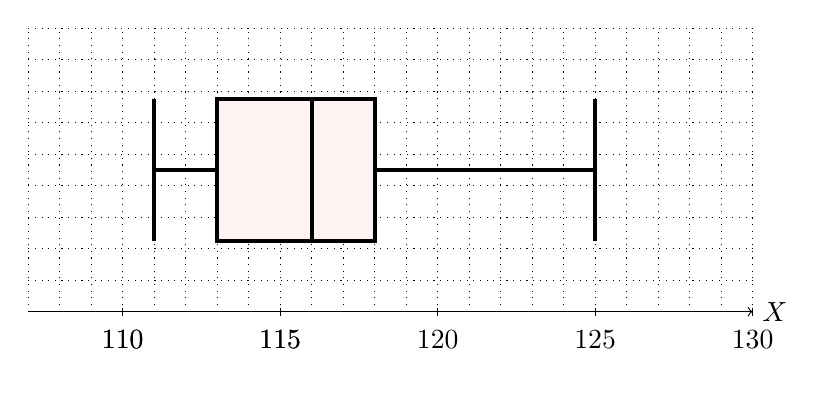
\begin{tikzpicture}[x=0.4cm,y=0.9cm]
         \draw[step=0.4cm,,dotted,color=black] (107,0) grid (130,4);
		\draw[->] (107,0) -- (130,0) node[right] {$X$} ;
		\foreach \X in {110,115,110,115,120,125,130} {
			\draw (\X,0.05cm) -- (\X,-0.05cm) node[below] {$\X\strut$};}
		\draw[ultra thick][fill=red!5] (113,1) rectangle (118,3);
  	\draw[ultra thick] (116,1) -- (116,3);

		\draw[ultra thick] (111,1) -- (111,3);
		\draw[ultra thick] (111,2) -- (113,2);
		\draw[ultra thick] (118,2) -- (125,2);
		%\draw[ultra thick] (4,1) -- (4,3);
		\draw[ultra thick] (125,1) -- (125,3);

			\end{tikzpicture}\\
	\end{center}



Quelle est cette erreur?

  \begin{checkboxes}
\choice La médiane n'est pas au bon endroit.  %  X1
\choice La moyenne échantillonnale n'est pas au bon endroit. % X_2 | X1
\choice Il devrait y avoir deux points: un à 105,5 et un à 125,5.
\choice La moustache de gauche devrait être à  105,5. 
\choice La moustache de droite devrait être à 125,5.
\choice Il y a plus qu'une erreur.
\choice Il n'y a aucune erreur.
\end{checkboxes}

\vspace{1cm}

\newpage




\question\label{conjointe}

Soit $X$ et $Y$ deux variables aléatoires dont la loi conjointe est 
$$f(x,y)=\left\{
			\begin{array}{ll}
   \displaystyle 4xye^{-(x^2+y^2)}  & \mbox{ si } x> 0\ \mbox{ et } \ y>0, \\
    0  & \mbox{ sinon. }
			\end{array}
			\right.$$



\begin{parts}
\part[6] Déterminez la densité marginale de $X$.

\begin{solution}
\begin{align*}
    \int_0^\infty 4xye^{-(x^2+y^2)} dy 
    &= -2xe^{-(x^2+y^2)} \big|_{y=0}^\infty \cr
    &= \frac{-2x}{e^{-(x^2+y^2)}}\big|_{y=0}^\infty  \cr
    &= 0 + \frac{2x}{e^{x^2}} \cr
    &= 2x e^{-x^2}
\end{align*}
La densité marginale est
$$f_X(x)=\left\{
			\begin{array}{ll}
   \displaystyle 2xe^{-(x^2)}  & \mbox{ si } x> 0, \\
    0  & \mbox{ sinon. }
			\end{array}
			\right.$$



    AUTRE SOLUTION: Ceux qui écrivent $f(x,y)=f(x)f(y)$ doivent justifier que le $f(x)$ et le $f(y)$ qu'ils ont trouvé est bien une densité, i.e. intègre à 1

    
\end{solution}

\vspace{10cm}

\part[5] Les variables aléatoires $X$ et $Y$ sont-elles indépendantes?

     \begin{oneparcheckboxes}
		\choice OUI
		\choice NON
\end{oneparcheckboxes}\\
{\bf Justification:}

\begin{solution}
    \begin{align*}
    \int_0^\infty 4xye^{-(x^2+y^2)} dx 
    &= -2ye^{-(x^2+y^2)} \big|_{x=0}^\infty \cr
    &= \frac{-2y}{e^{-(x^2+y^2)}}\big|_{x=0}^\infty  \cr
    &= 0 + \frac{2y}{e^{y^2}} \cr
    &= 2y e^{-y^2}
\end{align*}
On a donc que $f(x,y)=f(x)f(y)$, oui indépendance.
\end{solution}



\vfill



\end{parts}

\newpage




\question Soit le jeu de données $x_1,\hdots,x_n$, où $n$ est une nombre impair. Nous supposons que toutes les valeurs sont différentes. La moyenne échantillonnale de ce jeu de données est $\overline{x}$ et sa médiane est $\widetilde{x}$.
Dans chacune des situations suivantes, cochez toutes les réponses vraies.
\begin{parts}
    \part[2] Que pouvons-nous faire pour augmenter $\overline{x}$ sans augmenter $\widetilde{x}$?
    \begin{checkboxes}
        \choice Changer la valeur de $x_{(1)}$ pour une valeur supérieure à $x_{(n)}$
        \choice Changer la valeur de $x_{(n)}$ pour une valeur inférieure à $x_{(1)}$
        \correctchoice Changer la valeur de $x_{(n)}$ pour une valeur supérieure à $x_{(n)}$
        \correctchoice Changer la valeur de $x_{(1)}$ pour une valeur supérieure à $x_{(1)}$, mais inférieure à $\displaystyle x_{(0,5n + 0,5)}$
    \end{checkboxes}

    \part[2] Que pouvons-nous faire pour augmenter $\overline{x}$ et $\widetilde{x}$?
    \begin{checkboxes}
        \choice Changer la valeur de $x_{(1)}$ pour une valeur supérieure à $x_{(n)}$
        \choice Changer la valeur de $x_{(n)}$ pour une valeur inférieure à $x_{(1)}$
        \correctchoice Changer la valeur de $x_{(n)}$ pour une valeur supérieure à $x_{(n)}$
        \correctchoice Changer la valeur de $x_{(1)}$ pour une valeur supérieure à $x_{(1)}$, mais inférieure à $\displaystyle x_{(0,5n + 0,5)}$
    \end{checkboxes}
\end{parts}
\vspace{1cm}
\question[7] On a noté la fréquence cardiaque de neuf hommes. 
L'intervalle de confiance à 90\% obtenu pour la fréquence cardiaque moyenne est $[94; 112]$.
On suppose que la loi normale est adéquate pour cette variable aléatoire.

\vspace{0.25cm}
Déterminez si les énoncés suivants sont vrais ou faux. 

\textbf{\textit{Une bonne réponse vaut 1 point, une mauvaise réponse vaut -0,5 point et une réponse vide vaut 0 point, pour un total minimum de 0 point.}}

\vspace{0.25cm}
\begin{parts}
    \part La fréquence cardiaque moyenne des hommes ayant participé à l'étude est de 103 battements par minute.
    
    \begin{oneparcheckboxes}
        \choice Vrai
        \choice Faux
    \end{oneparcheckboxes}
\vspace{0.25cm}

    \part Si on recommençait la même expérience avec neuf autres individus de la même population, il y aurait 90\% de chances que la nouvelle moyenne échantillonnale soit comprise entre 94 et 112.
    
    \begin{oneparcheckboxes}
        \choice Vrai
        \choice Faux
    \end{oneparcheckboxes}
\vspace{0.25cm}

    \part Environ 90\% des hommes de cette population ont une fréquence cardiaque comprise entre 94 et 112.
    
    \begin{oneparcheckboxes}
        \choice Vrai
        \choice Faux
    \end{oneparcheckboxes}
\vspace{0.25cm}

    \part Environ 90\% des hommes de cet échantillon ont une fréquence cardiaque comprise entre 94 et 112.
    
    \begin{oneparcheckboxes}
        \choice Vrai
        \choice Faux
    \end{oneparcheckboxes}
\vspace{0.25cm}

    \part La probabilité que la moyenne échantillonnale soit comprise entre 94 et 112 est 90\%.
    
    \begin{oneparcheckboxes}
        \choice Vrai
        \choice Faux
    \end{oneparcheckboxes}
\vspace{0.25cm}

    \part La probabilité que la moyenne de la population soit comprise entre 94 et 112 est 90\%.
    
    \begin{oneparcheckboxes}
        \choice Vrai
        \choice Faux
    \end{oneparcheckboxes}
    \vspace{0.25cm}

    \part Si on avait utilisé un échantillon de 50 individus, l'intervalle de confiance aurait probablement été plus court.
    
    \begin{oneparcheckboxes}
        \choice Vrai
        \choice Faux
    \end{oneparcheckboxes}
    \vspace{0.25cm}


    
\end{parts}
\newpage

\question[8] Soit la variable aléatoire $X$ et sa fonction de répartition

\[ F(x) =
\begin{cases}
   \displaystyle 1-e^{-(x/\beta)^\alpha}& \text{si } x \ge 0, \\
    0 & \text{sinon},
\end{cases}
\]
où $\alpha$ et $\beta$ sont des constantes connues.

En posant $\alpha = 2$ et $\beta=0,5$, calculez $P(X\geq \sqrt{3} | X\geq \sqrt{2})$.

\begin{solution}
    \begin{align*}
        \frac{P(X \geq \sqrt{3} \cap X \geq \sqrt{2})}{P(X \geq \sqrt{2})}
        &= \frac{P(X \geq \sqrt{3} }{P(X \geq \sqrt{2})} \cr
        &=\frac{1-F(\sqrt{3})}{1-F(\sqrt{2})} \cr
        &=\frac{e^{-(\sqrt{3}/0,5)^2}}{e^{-(\sqrt{2}/0,5)^2}}\cr
        &= \frac{e^{-3/0,25}}{e^{-2/0,25}} \cr
        &= e^{2 \times 4}e^{-3\times 4} \cr
        &= e^{8-12} = e^{-4}
    \end{align*}
\end{solution}



\newpage
\question\label{estimateursPonctuels} 
Soit $X_1,\hdots,X_9$ des réalisations indépendantes d'une variable $X\sim\mathcal{N}(\mu, 4)$. 

\begin{parts}
    \part[5] Calculez $P(\overline{X}>\mu+0,62S)$. 
    
    \begin{solution}
        \begin{align*}
            P(\overline{X} > \mu + 0,62S)
            &= P(\overline{X} - \mu  > 0,62S) \cr
             &= P\left(\frac{\overline{X} - \mu}{S/\sqrt{n}}  >  \frac{0,62 S}{S/\sqrt{n}}\right) \cr
             &= P\left( T_{n-1} >  0,62 {\sqrt{9}}\right) \cr
             &= P\left( T_{8} > 1,86\right) \cr
             &= 0,05
        \end{align*}
    \end{solution}
\vspace{10cm}
    \part[5] Calculez la probabilité que la variance échantillonnale soit supérieure à 8,765.

    
        \begin{solution}
        \begin{align*}
            P(S^2 > 8,765)
             &= P\left(\frac{(n-1)S^2}{\sigma^2}  > \frac{(n-1)8,765}{\sigma^2}\right) \cr
             &= P\left( \chi_{n-1}^2  > \frac{8\times 8,765}{4}\right) \cr
             &= P\left( \chi_{8}^2  > 17,53\right) \cr
             &= 0,025
        \end{align*}
    \end{solution}
\end{parts}
\newpage

\question[8]
Un producteur de Gruyère sait que le poids d'une de ses meules de fromage, $X$, est une variable aléatoire d'espérance $\mu=30$ kg et de variance $\sigma^2 = 9$ kg$^2$. Il doit envoyer 144 meules à un festival. Le transporteur lui chargera 1500\$, à condition que le poids moyen des 144 meules soit inférieur ou égal à $30,5$ kg. Dans le cas contraire, il lui chargera 2000\$.

Quelle est la probabilité approximative que le transporteur lui charge 1500\$?
    \vspace{12cm}

\begin{solution}
    \begin{align*}
        E(X) &= 30 \cr
        V(X) &= 9 \cr
        n&= 144 \cr
        \overline{X} &\approx N(30, 9/144) \cr
        1500 \$ \; &si \; \overline{X} \leq 30,5 \cr
        2000 \$ \; &si \; \overline{X} \geq 30,5 
    \end{align*}

    \begin{align*}
        P\left( \overline{X} \leq 30,5 \right)
        &= P\left( \frac{\overline{X}-30}{\sqrt{9/144}} \leq \frac{30,5-30}{\sqrt{9/144}}  \right) \cr
        &\approx P\left( Z \leq \frac{0,5}{\sqrt{3/12}}  \right) \cr
        &= P\left( Z \leq 2 \right) \cr
        &= \Phi(2) \cr
        &= 0,97725
    \end{align*}
\end{solution}

\newpage



\newpage

\question On veut calibrer une certaine machine pour qu'elle soit le plus stable possible.
On veut d’abord estimer la variation de la taille des pièces produites à l'aide d'un intervalle de confiance, en supposant que la loi normale modélise bien la variable aléatoire en question.
Un échantillon de taille 16 a donné une variance échantillonnale de 150 cm$^2$.
La borne inférieure de l'intervalle de confiance pour la variance est $90$.

\vspace{0.5cm}
\begin{parts}
    \part[6] Quel est le niveau de l'intervalle de confiance?

\begin{solution}
    \begin{align*}
        b_{inf} &= \frac{(n-1)S^2}{\chi_{\alpha/2;n-1}} \cr
        90 &= \frac{15 \times 150}{\chi_{\alpha/2;n-1}} \cr
        \chi_{\alpha/2;n-1} &= \frac{150}{6}  \cr
        \chi_{\alpha/2;15} &= 25 \cr
        \alpha/2 &= 0,05 \cr
        \alpha &= 0,10
    \end{align*}
\end{solution}
    
    \vspace{12 cm}
    \part[4] Que vaut la borne supérieure de l'intervalle de confiance?


    \begin{solution}
    \begin{align*}
        \frac{(n-1)S^2}{\chi_{1-\alpha/2;n-1}} 
         &= \frac{15 \times 150}{\chi_{1-\alpha/2;15}} \cr
        &= \frac{15 \times 150}{\chi_{0,95;15}}  \cr
        &= \frac{15 \times 150}{7,26}\cr
        &= 309,92
    \end{align*}
\end{solution}


\end{parts}




\end{questions}

\end{document} 
